\documentclass[final,hyperref={pdfpagelabels=false}]{beamer}
\mode<presentation>
  {
  \usetheme{Berlin}
  %\usetheme{Dreuw}
  }
  \usepackage{times}
  \usepackage{amsmath,amsthm, amssymb, latexsym}
  \boldmath
  \usepackage{exscale}
  \usepackage[english]{babel}
  \usepackage[latin1]{inputenc}
  \usepackage[orientation=portrait,size=a0,scale=1.4,debug]{beamerposter}
  \usepackage{ragged2e} 
  \renewcommand\baselinestretch{1.08} 

  %%%%%%%%%%%%%%%%%%%%%%%%%%%%%%%%%%%%%%%%%%%%%%%%%%%%%%%%%%%%%%%%%%%%%%%%%%%%%%%%%5
  \graphicspath{{figures/}}
  \title{How to optimize the parameters of the\\Smooth Particle Mesh Ewald algorithm}
  \author{Han Wang \inst{1}, Florian Dommert \inst{2}, Christian Holm \inst{2}}
  \institute[]{ \footnotesize
    \inst{1} LMAM and School of Mathematical Sciences, Peking University, \textit{Beijing}, China  \\
    \inst{2} Institute for Computational Physics, Universit\"at Stuttgart, \textit{Stuttgart}, Germany
  }
  %\date{Jul. 31th, 2007}
%  \RequirePackage{tangocolors}
%  \setbeamercolor{headline}{fg=black,bg=tagray}

  %%%%%%%%%%%%%%%%%%%%%%%%%%%%%%%%%%%%%%%%%%%%%%%%%%%%%%%%%%%%%%%%%%%%%%%%%%%%%%%%%5
  \begin{document}
    
  \newcommand{\redc}[1]{{\color{red} #1}}
  \newcommand{\bluec}[1]{{\color{blue} #1}}
  \renewcommand{\v}[1]{\textbf{\textit{#1}}}
  \renewcommand{\d}[1]{\textrm{#1}}


  \begin{frame}{} 
    \vfill
    \begin{beamercolorbox}[wd=\paperwidth]{headline}
      \begin{columns}[T]
        \begin{column}{.2\paperwidth}
          \begin{center}
            \hspace{4ex}
\includegraphics[width=.5\linewidth]{logo/pku.png}
          \end{center}
        \end{column}
        \begin{column}{.6\paperwidth}
          \vskip1ex
          % \raggedleft
          \centering
          \usebeamercolor{title in headline}{\color{fg}\textbf{\LARGE{\inserttitle}}\\[1ex]}
          \usebeamercolor{author in headline}{\color{fg}\large{\insertauthor}\\[1ex]}
          \usebeamercolor{institute in headline}{\color{fg}\large{\insertinstitute}\\[1ex]}     
          \vskip4ex
        \end{column}
        \begin{column}{.2\paperwidth}
          \begin{center}
            \vspace*{-1em}
            \hspace{-2ex}\includegraphics[width=.4\linewidth]{logo/unilogo}\\
            \vspace*{0.5em}
            \hspace{-2ex}\includegraphics[width=.6\linewidth]{logo/Logo_ICP_T_V2}
            \vfill
          \end{center}
        \end{column}
      \end{columns}
    \end{beamercolorbox}

    \vfill
    \vspace{-1cm}
    \begin{columns}[t]
      \begin{column}{.32\linewidth}
        \vfill
        \begin{block}{\large Abstract}
          \vspace{1ex}
          \begin{minipage}[c]{.975\linewidth}
          We derive an error estimate for the smooth Particle Mesh Ewald~(SPME)
          algorithm, which is often used for Molecular Dynamics simulations, and
          applied it to an ionic system to test its va\-lid\-i\-ty. Various
          combinations of parameters were tested for two different
          implementations of the SPME algorithm to proof the quality of the
          estimate, resulting in a parameter tuning algorithm for SPME.
        \end{minipage}
        \end{block}
        \vfill
        \begin{block}{\large Electrostatic energy}
          \vspace{1ex}
          \begin{minipage}[c]{.975\linewidth}
          The electrostatic energy of a periodic ionic system is 
          \begin{equation*}\bluec{ E = \frac12
              \sum^\ast_{n}\sum_{i,j}\frac{q_i q_j}{\vert \v r_{ij} +
                \v n\vert},}
          \end{equation*} 
          and the essential difficulty to apply this formula follows from its 
          \redc{``long range''} nature.
          \vspace*{-1.2ex}
          \begin{figure}
            \centering 
            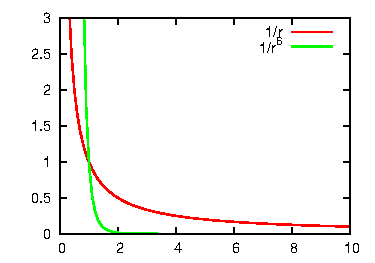
\includegraphics[width=0.75\textwidth]{figs/decay.pdf}
          \end{figure}
          \vspace*{-1.5ex}
        \end{minipage}
        \end{block}
        \vfill
        \begin{block}{\large Ewald summation}
          \vspace{1ex}
          \begin{minipage}[c]{.975\linewidth}
          A good way to deal with the electrostatic in\-ter\-action in periodic
          systems was proposed by Ewald in 1921:
          \begin{align*}
            E &=  E_{\textrm{dir}} +E_{\textrm{rec}}+E_{\textrm{corr}}\\
            E_{\textrm{dir}} & = \frac12 \sum^{\ast}_{\v n}
            \sum_{i,j = 1}^{N} \frac{q_iq_j\, \redc{\textrm{erfc}(\beta \vert\v{r}_{ij} + \v{n}\vert)}}
            {\vert\v{r}_{ij} + \v{n}\vert} \\ \label{Erec-ewald}
            E_{\textrm{rec}} & = \frac1{2\pi V} \sum_{\v m \neq 0}
            \frac{\redc{\exp(-\pi^2\v m^2 / \beta^2)}}{\v m^2} S(\v m) S(-\v m) \\
            E_{\textrm{corr}}& = -\frac\beta{\sqrt \pi} \sum_{i=1}^N q_i^2
          \end {align*}
          Consider the \redc{``short range''} nature of the red terms in both real and
          reciprocal space, and the structure factor $S(\v m)$ given by:
          \begin{equation*}
            S(\v m) = \sum_{j=1}^N q_j \exp (2 \pi i \v m \cdot \v r_j).
          \end{equation*}
          Unfortunately, the computational cost is \redc{$\mathcal O(N^{3/2})$}
          at the best.          
        \end{minipage}
        \end{block}
        \vfill
        \begin{block}{\large $O(N \log N)$ algorithms}
          \vspace{1ex}
          \begin{minipage}[c]{.975\linewidth}
          In the last two decades, some successful algorithms have
          been developed: 
          \begin{itemize}
          \item The \redc Particle--\redc Particle--\redc Particle--\redc Mesh method
          \item The \redc Particle \redc Mesh \redc Ewald method 
          \item The \redc Smooth \redc Particle \redc Mesh \redc Ewald method 
          \end{itemize}

          \bluec{\textbf{Key point:}} The term $ \exp (2 \pi i
          \v m \cdot \v r_j) $ is just calculated on a given number of grid
          points. To derive its value at any other position, an interpolation is 
          using the known values on the neighboring grid points. Therefore 
          Fast Fourier transforms (FFT) can be applied for the calculation of
          the reciprocal part and the computational cost is drastically
          decreased to \redc{$\mathcal O(N\log N)$}.
        \end{minipage}
        \end{block}
      \end{column}
      \begin{column}{.32\linewidth}
        \vfill
        \begin{block}{\large The parameters in SPME}
          \vspace{1ex}
          \begin{minipage}[c]{.975\linewidth}
          \begin{itemize}
          \item \bluec{$\beta$} corresponds to the same parameter as in the Ewald summation.
          \item \bluec{$r_c$} is the cut off used in the neighbor list method
            for the direct part.
          \item \bluec{$n$}  defines the order of the cardinal B-splines.
          \item \bluec{$\v K$}  contains the number of grid points used to
            discrete the space in every dimension.
          \end{itemize}
          It is not a prior clear how to choose these parameters properly, but
          an arbitrary choice may lead to \redc{totally wrong results}.
          
          When using SPME method, there are two possible ways of
          calculating forces in the charged system, that differ in the
          computational effort and accuracy, considering the same set of
          parameters.
          \vspace*{-0.5ex}
          \begin{itemize}
            \item \bluec{ik differentiation}\vspace{0.4ex}
              \begin{minipage}{0.975\textwidth} 
                Multiplying the reciprocal energy with the vector \bluec{$ik$} in
                reciprocal space, and transforming the result back to real
                space corresponds to a derivative and yields the force. However
                \redc{4} FFTs are required, but momentum is \redc{conserved}.
              \end{minipage}\vspace*{0.2ex}
            \item \bluec{analytical differentiation}\vspace{0.4ex}
            \begin{minipage}{0.975\textwidth}
            The forces are derived from the the derivative of the approximated
            energy. Only \redc{2} FFTs are required, but momentum is \redc{not}
            conserved.
            \vspace*{-0.2ex}
        \end{minipage}
          \end{itemize}
        \end{minipage}
        \end{block}
        \vfill
        \begin{block}{\large Designing a parameter tuning algorithm}
          \vspace{1ex}
          \begin{minipage}[c]{.975\linewidth}
          To tune the parameters, we need:
          \begin{itemize}\justifying
          \item \bluec{Error estimates} that ensure the algorithm to give
            correct results. 
          \item \bluec{CPU-time estimates} that yield the most time-saving
            parameters for a given allowed error.
          \end{itemize}
        \end{minipage}
        \end{block}
        \begin{block}{\large CPU-time estimate}
          \vspace{1ex}
          \begin{minipage}[c]{.975\linewidth}
          \begin{itemize}
          \item Direct part \quad \redc{$T^{\textrm{dir}} \approx
              C_dr_c^3$}
          \item Reciprocal part 
            \begin{itemize}
            \item ik differentiation \newline
              \redc{$
                T^{\textrm{rec}}_{\textrm{ik}}
                \approx 2 C_s Nn^3 + 4\, C_f  K_1K_2K_3 \log (K_1K_2K_3) 
                $}
            \item analytical differentiation\newline
              \redc{$
                T^{\textrm{rec}}_{\textrm{ana}}
                \approx 3C_s Nn^3 + 2\, C_f  K_1K_2K_3 \log (K_1K_2K_3).
                $}
            \end{itemize}
          \end{itemize}
        \end{minipage}
        \end{block}
        \vfill
        \begin{block}{\large Error estimates}
          \vspace{1ex}
          \begin{minipage}[c]{.975\linewidth}
          As a measure the root mean square (RMS) force error is widely used:
          $$ \bluec{\varepsilon(r_c, \v K,
            n, \beta) = \sqrt{\langle(\v F^{\textrm{exact}} - \v
              F^{\textrm{{approx}}})^2\rangle} },$$
          with $\v F^{\d {exact}}$ and $\v F^{\d {approx}}$ denoting the
          exact forces and interactions derived with the SPME,
          respectively, and estimated in direct~(green) and
          reciprocal space~(blue) independently.
          \vspace{-1ex}
          \begin{figure}
            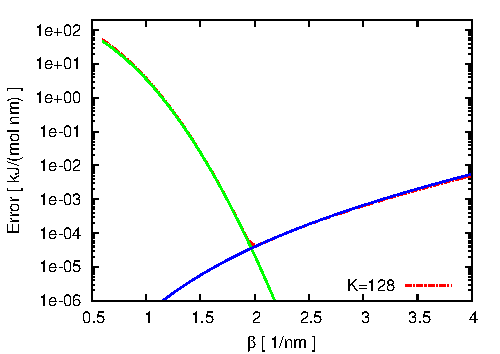
\includegraphics[width=0.9\textwidth]{figs/bspline-order6.pdf}
          \vspace{-1ex}
            \caption{The actual and estimated error resulting from the ik
              differentiation scheme as a function of $\beta$ at a fixed order
              $n=6$ }
          \end{figure}
        \end{minipage}
          \vspace{-0.4ex}
        \end{block}
      \end{column}
      \begin{column}{.32\linewidth}
        \vfill
        \begin{block}{\large Error estimates}
          \begin{minipage}[c]{.975\linewidth}
        \begin{figure}
          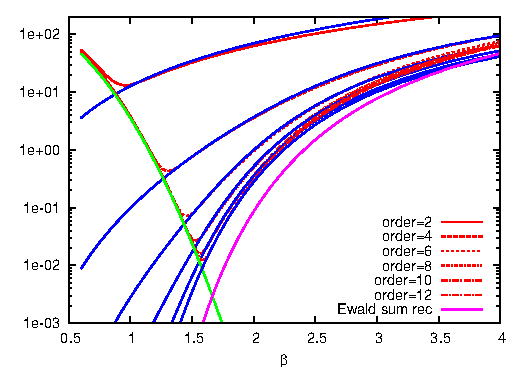
\includegraphics[width=0.95\textwidth]{figs/bspline-mesh32.pdf}
          \caption{The actual and estimated error as a
          function of $\beta$ resulting from the ik
          differentiation scheme when applying a fixed grid size of $\v K = (32, 32, 32)$ .}  
        \end{figure} 
        \end{minipage}
        \end{block}
        \vfill
        \begin{block}{\large Parameter tuning}
          \vspace{1ex}
          \begin{minipage}[c]{.975\linewidth}
          From the mathematical point of view, the parameter tuning
          problem is a constrained optimization problem:\bluec{
            \begin{align*} 
              \min\quad &  T (r_c, \v K, n, \beta),\\
              \textrm{\textbf{s.t.}}\quad & \varepsilon (r_c, \v K, n, \beta) \leq \varepsilon^\ast
            \end{align*}}The interpolation order $n$ is restricted to $ 2, 4, 6, 8$ and
          $K_\alpha$ should be able to decompose into small prime
          numbers, such as 2, 3, 5 and 7. We solve this problem by
          \redc{a splitting strategy}, that implies solving the following two
          problems independently \bluec{
          \begin{align*}
            (1) & \left\{
          \begin{aligned}
            \min\quad & 
            T^{\textrm{dir}} (r_c, \beta_0), \\* 
            \textrm{\textbf{s.t.}}\quad & 
            \varepsilon^{\textrm{dir}} (r_c, \beta_0) \leq \varepsilon^\ast_{\textrm{dir}},
          \end{aligned}\right. \\ 
          (2) & \left\{\begin{aligned}
            \min\quad & 
            T^{\textrm{rec}} (\v K, n, \beta_0), \\* 
            \textrm{\textbf{s.t.}}\quad & 
            \varepsilon^{\textrm{rec}} (\v K, n, \beta_0) \leq \varepsilon^\ast_{\textrm{rec}},
          \end{aligned}\right.
        \end{align*}}
        by the \redc{bisection method}. The splitting parameter $\beta_0$ is
        finally derived by the \redc{0.618 searching method}.
        \vspace{-1.9ex}
          \begin{figure}
            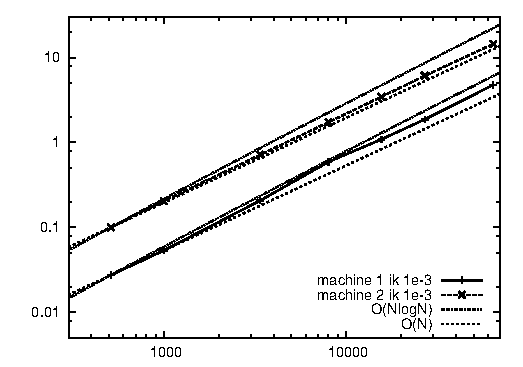
\includegraphics[width=0.85\textwidth]{figs/both-time-1e-3.pdf}
        \vspace{-1ex}
            \caption{Computational cost of ik differentiated SPME
              method as a function of particle number. The target
              precision is $\varepsilon^\ast=10^{-3}$.}
        \vspace{-1ex}
          \end{figure}
        \end{minipage}
        \end{block}
        \begin{block}{\large Further findings}
          \vspace{1ex}
          \begin{minipage}[c]{.975\linewidth}
          \begin{itemize}
%           \item The error estimation is proved to be sharp.
%           \item We demonstrate the parameter tuning algorithm produces
%             reasonable parameters for SPME.
          \item\justifying For the tested machines, there is \redc{no
              significant difference} between ik and analytical
            differentiation regarding precision and CPU time. The
            analytical differentiation, however lacks momentum
            conservation, a deficiency that has to be removed in order
            to avoid spurious drifts.
          \item The parameters $r_c, n, \beta$ only depend on the charge
            density, target precision and used machine,
            and do \redc{NOT} depend on the size of system~$N$. However the
            value $K_1K_2K_3$ is roughly \redc{proportional} to $N$. 
            \redc{Therefore we can tune the parameters for one reference system and derive
              parameters any system based on the reference system.}
          \end{itemize}
        \end{minipage}
        \vspace{-0.15ex}
        \end{block}
%         \begin{block}{Emails}
%           \texttt{han\_wang@math.pku.edu.cn} \\
%           \texttt{dommert@icp.uni-stuttgart.de} \\
%           \texttt{holm@icp.uni-stuttgart.de}
%         \end{block}
      \end{column}
    \end{columns}
        \vfill
  \end{frame}
\end{document}


%%%%%%%%%%%%%%%%%%%%%%%%%%%%%%%%%%%%%%%%%%%%%%%%%%%%%%%%%%%%%%%%%%%%%%%%%%%%%%%%%%%%%%%%%%%%%%%%%%%%
%%% Local Variables: 
%%% mode: latex
%%% TeX-PDF-mode: t
%%% End:
